\chapter{Plasma Model}
\section{Four-temperature Plasma Model}
The temperature of the jet plasma cools down as it goes farther from the accretor. To obtain a more physical understanding of the the X-ray spectra, we use a plasma diagnostic approach where emission lines correspond to four specific jet plasma temperatures \citep{Marshall2002}. Eastern and Western jets are fitted at the same time using this four-temperature plasma model. The parameters of the model for each jet are absorption column density, four normalizations that are related to the emission measure of the plasma, four temperatures, electron density $n_e$, velocity of turbulence, redshift, metal abundance, and Ni abundance. Since two jets are assumed to share the same properties, all the parameters except redshifts and normalizations are tied together. Since the jet emits at a fast  speed of 0.26 $c$ and the time for speed and the time for the particles travelling through the X-ray part of the jet is short, we assume that the electron densities $n_e$ of the four components are the same. \par 

The observed flux of an emission line from a region of plasma with electron density $n_e$ and temperature $T$ is given by

\begin{equation*}
    f_i = \dfrac{J_i(T)\int n_en_H dV }{4\pi D^2} = \dfrac{J_i(T)EM(T)}{4\pi D^2}
\end{equation*}
where D is the distance from the Earth to the source, in our case, 5.5 kpc, $n_H$ is the density of the hydrogen and EM is the emission measure.\par 

EM can be found using the definition of normalizations in the default plasma function in ISIS,
\begin{equation*}
    \mathrm{norm} = \dfrac{1\times 10^{-14}}{4\pi D^2}\int n_e n_H dV =  \dfrac{1\times 10^{-14}}{4\pi D^2} EM
\end{equation*}




\section{The 20 ksec observation}
The HEG and MEG spectra were modeled jointly using ISIS and the APED atomic data base on line emissivities and ionization balance. The fitted model spectra are shown in Fig~\ref{plasma_short1} - Fig~\ref{plasma_short3}. Table~\ref{tab:plasma} shows the result of plasma model fitting.\par 

The interstellar medium (ISM) absorption $N_H = (1.57 \pm 0.0024) \times 10^{22}$ $\mathrm{cm^{-2}}$. $N_H$ is the column density of neutral hydrogen, which is typically due to H-atoms between us and the source. However, for sources like SS 433, some fraction of $N_H$ could be due to H-atoms presenting near the binary system itself. The parameters of plasma model is in Table~\ref{tab:plasma}, where $n_e$ is the electron density, metal is the metal abundance relative to solar, Ni is the Ni abundance relative to solar and EM is the emission measure. 


% Given that ions existing in different temperature
% ranges have similar line widths and Doppler shifts, we assume that the flow has a constant opening angle and jet velocity.

\begin{deluxetable}{rcccccc}
\tablecolumns{5}
\tablewidth{0pc}
\tabletypesize{\small}
\tablecaption{Jet Parameters from a Multitemperature model for the 20 ksec observation
\label{tab:plasma} }
\tablehead{& & & & &Western jet & Eastern jet\\
\colhead{T} &  \colhead{$n_e$} &  \colhead{vturb} & \colhead{metal} & \colhead{Ni} & \colhead{EM} & \colhead{EM} \\
  \colhead{($\times 10^6$ K)}  & \colhead{($\times 10^{14} \mathrm{cm^{-3}}$)}& \colhead{(km/s)} &\colhead{($\odot$ metal)} & \colhead{($\odot$ Ni)} & \colhead{($\times 10^{57}\mathrm{cm^{-3}}$)} & \colhead{($\times 10^{57}\mathrm{cm^{-3}}$)}}
\startdata
6.3& 1 & 1876.6 & 3.086 & 42.61 & 1.86 &  1.29 \\
12.6& 1 & 1876.6& 3.086 & 42.61 & 2.09 &  $<$0.037 \\ 
31.6& 1 & 1876.6& 3.086 & 42.61 & $<$0.037 &  $<$0.037 \\
126.& 1 & 1876.6& 3.086 & 42.61 & 10.42 &  14.16 \\
\enddata
\end{deluxetable}


\begin{figure}
    \centering
    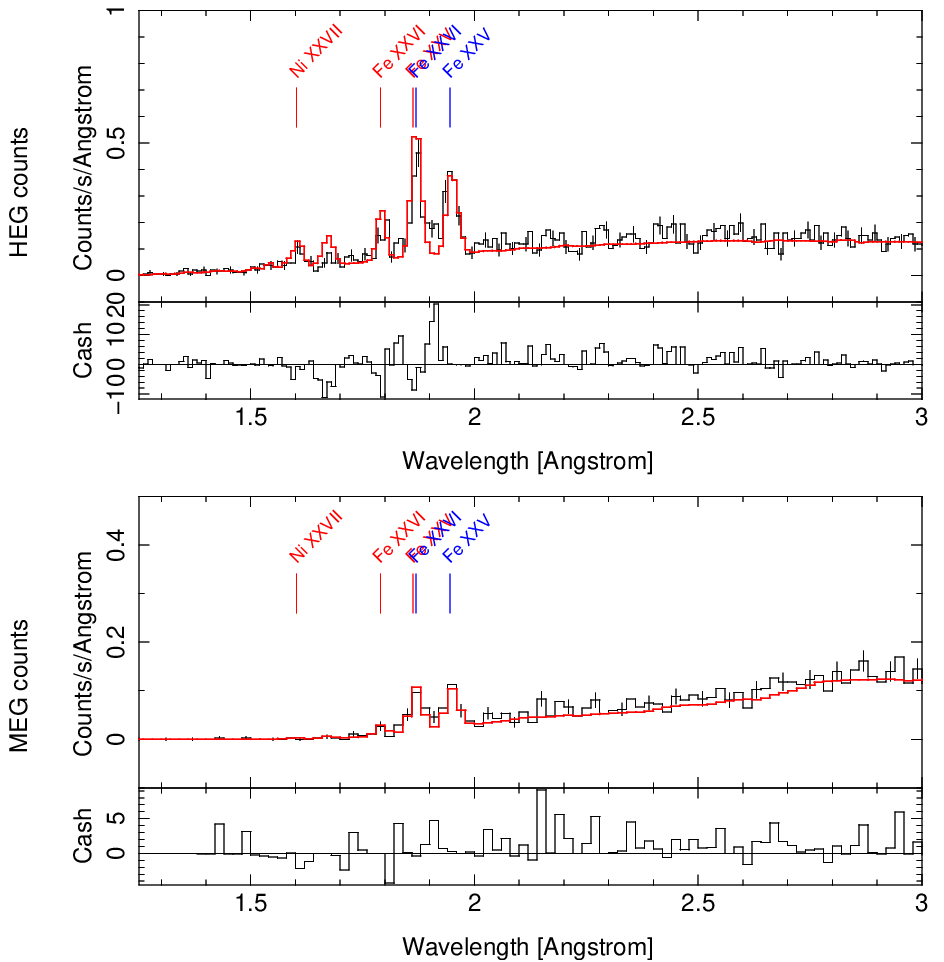
\includegraphics[width = \linewidth]{Chapters/Figures/plasma_short1.png}
    \caption{The 1.25-3.0 \AA\ regions of the HEG (top) and MEG (bottom) spectra of SS 433 observed with the Chandra HETGS on 2018 August 10, compared to a plasma model of the spectra of the blue and red jets. Black line: observed spectrum. Red line: four temperature plasma model providing a generally adequate fit to the spectrum. Line identifications are labeled where there are features in the spectrum and confirmed by the model. The red characters label the emission lines from the Western jet while the blue ones from the Eastern jet. The Cash statistic residuals are shown at the bottom of each spectrum. Fe {\sc xxvi} from the Eastern jet and Fe {\sc xxv} from the Western jet are blended. }    \label{plasma_short1}
\end{figure}


\begin{figure}
    \centering
    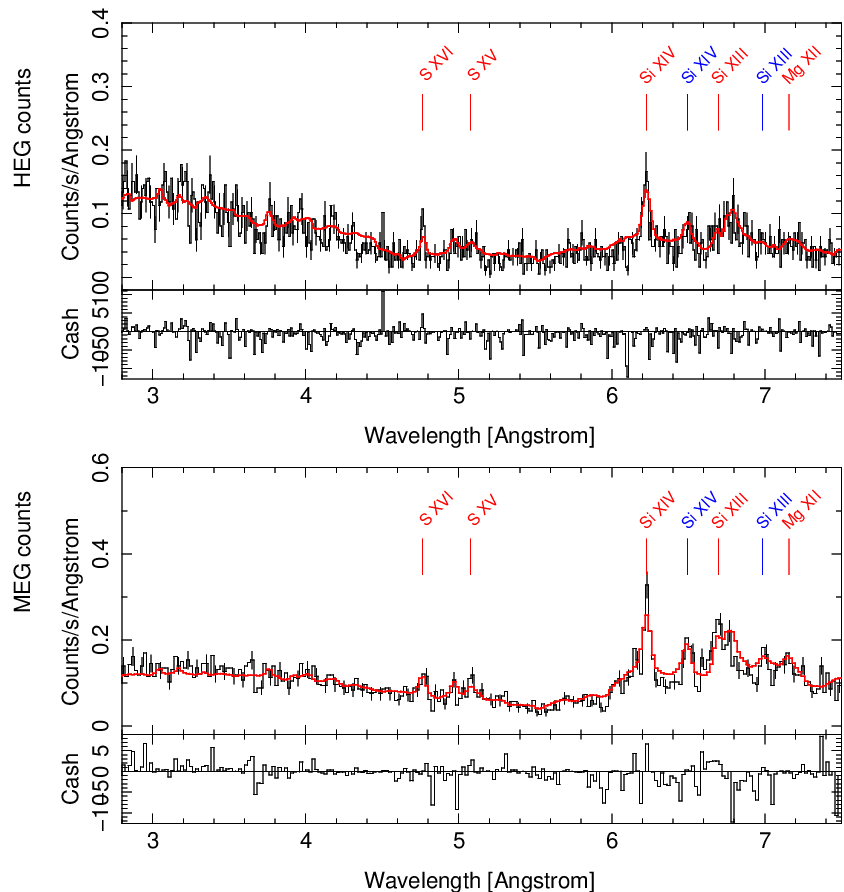
\includegraphics[width = \linewidth]{Chapters/Figures/plasma_short2.png}
    \caption{Same as Figure~\ref{plasma_short1}, except for the 2.8-7.5 \AA\ region. Si {\sc xiv} and Si {\sc xiii} are well fit.}
    \label{plasma_short2}
\end{figure}

\begin{figure}
    \centering
    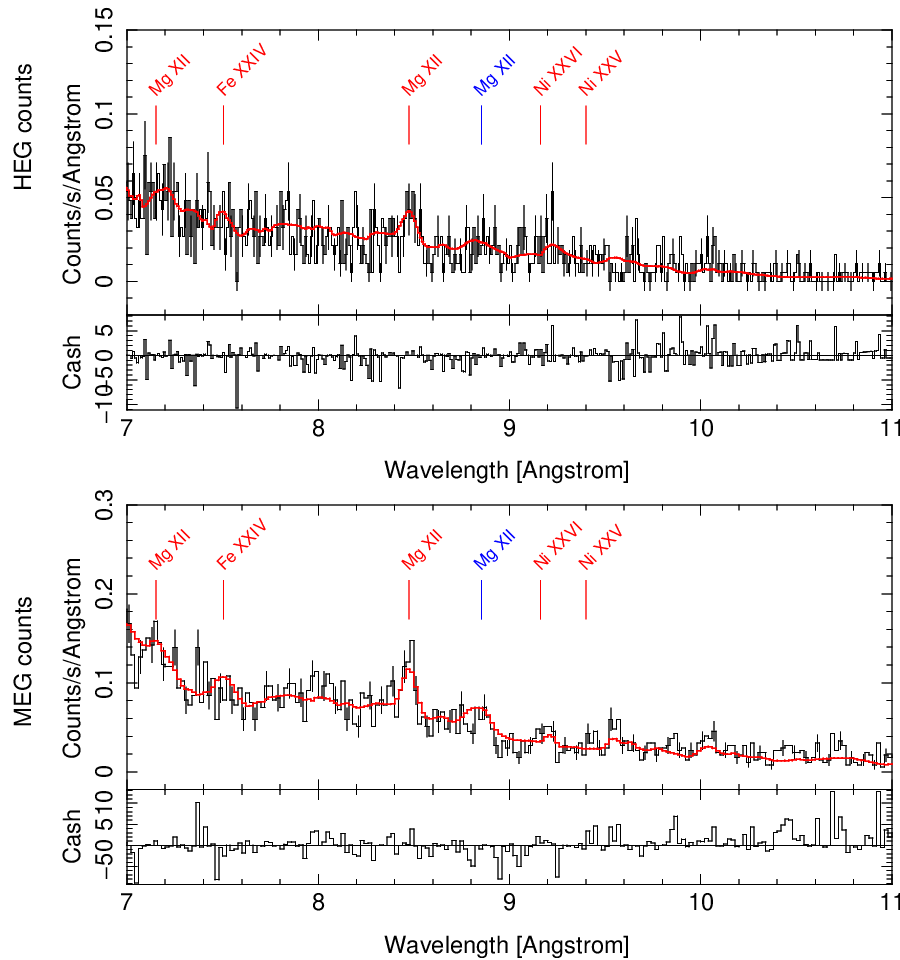
\includegraphics[width = \linewidth]{Chapters/Figures/plasma_short3.png}
    \caption{Same as Figure~\ref{plasma_short2}, except for the 7-11 \AA\ region. }
    \label{plasma_short3}
\end{figure}


\newpage
\section{The 96 ksec Observation}

Using the similar fitting routine as the short observation, the four-temperature plasma model fit the whole long observation. The interstellar medium (ISM) absorption $N_H = (1.23 \pm 0.0024) \times 10^{22}$ $\mathrm{cm^{-2}}$.\par 


Figure~\ref{long_plasma1} - \ref{long_plasma3} shows that highly ionized iron lines from the Eastern jet were occulted during the eclipse and silicon lines from the receding (Eastern) jet also appeared fainter. This suggests that both the hot and cool part of the Eastern jet were likely occulted by the companion star. Given that ions which exist in different temperatures has a similar width and redshift, we assume that the flow has a constant jet velocity and opening angle. 
Table~\ref{tab:plasma_long} shows the results of the four-temperature plasma model for the long observation. Comparing with the plasma model results for the short observation, it is noticeable that the metal abundance (Fe, S, Si, Mg) decreased by 9.6\% and Ni abundance decreased by 29\%. The emission measures of the Eastern jet in the $126 \times 10^6$ K temperature region decreased significantly by 74\% before and during the eclipse. This matches with the spectrum, showing the disappearance of Fe {\sc xxvi} and faint lines from the Eastern jet due to the eclipse. 









\begin{figure}
    \centering
    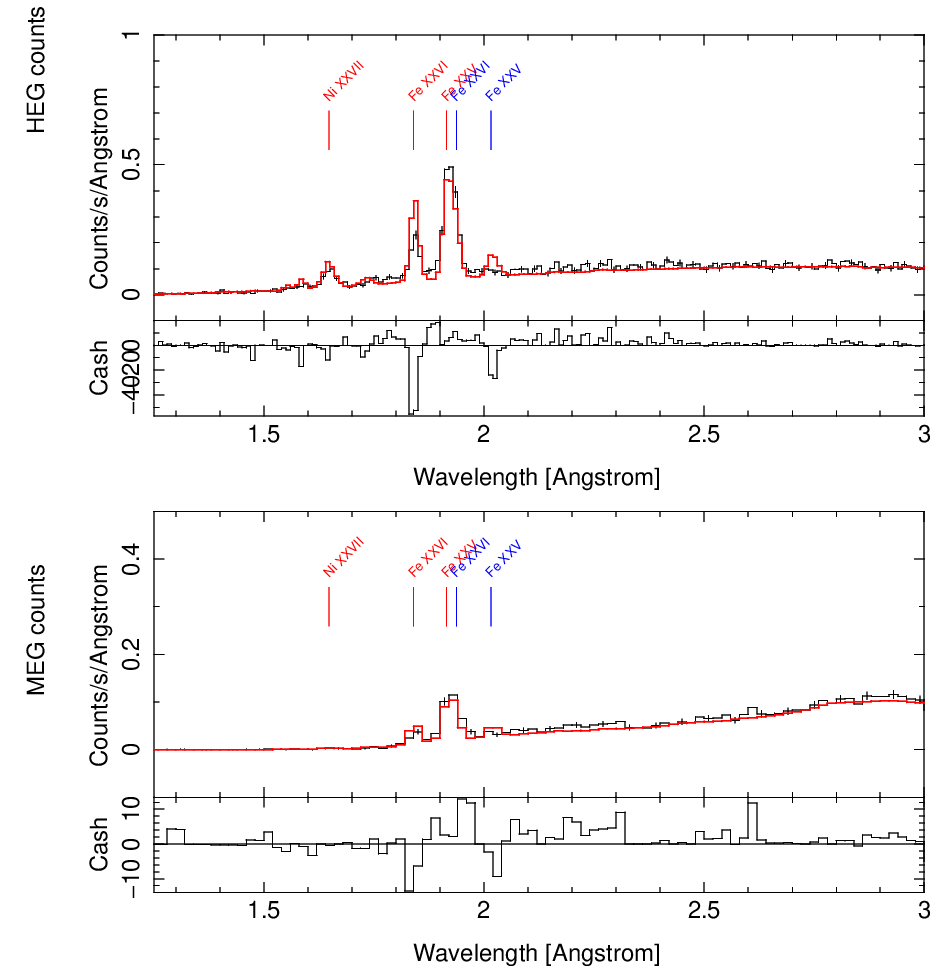
\includegraphics[width = \linewidth]{Chapters/Figures/long_plasma_whole1.png}
    \caption{The 1.25-3.0 portions of the HEG and MEG spectra of SS 433 observed with the Chandra HETGS during 2018 August 13 - 14, compared to a model of the spectra of the blue and red jets. Red line: four temperature plasma model providing a generally adequate fit to the spectrum. Line identifications are labeled where there are features in the spectrum and confirmed by the model. The red characters label the emission lines from the Western jet while the blue ones from the Eastern jet. The Cash statistic residuals are shown at the bottom of each spectrum. Fe {\sc xxvi} from the Eastern jet and Fe {\sc xxv} from the Western jet are blended.}
    \label{long_plasma1}
\end{figure}

\begin{figure}
    \centering
    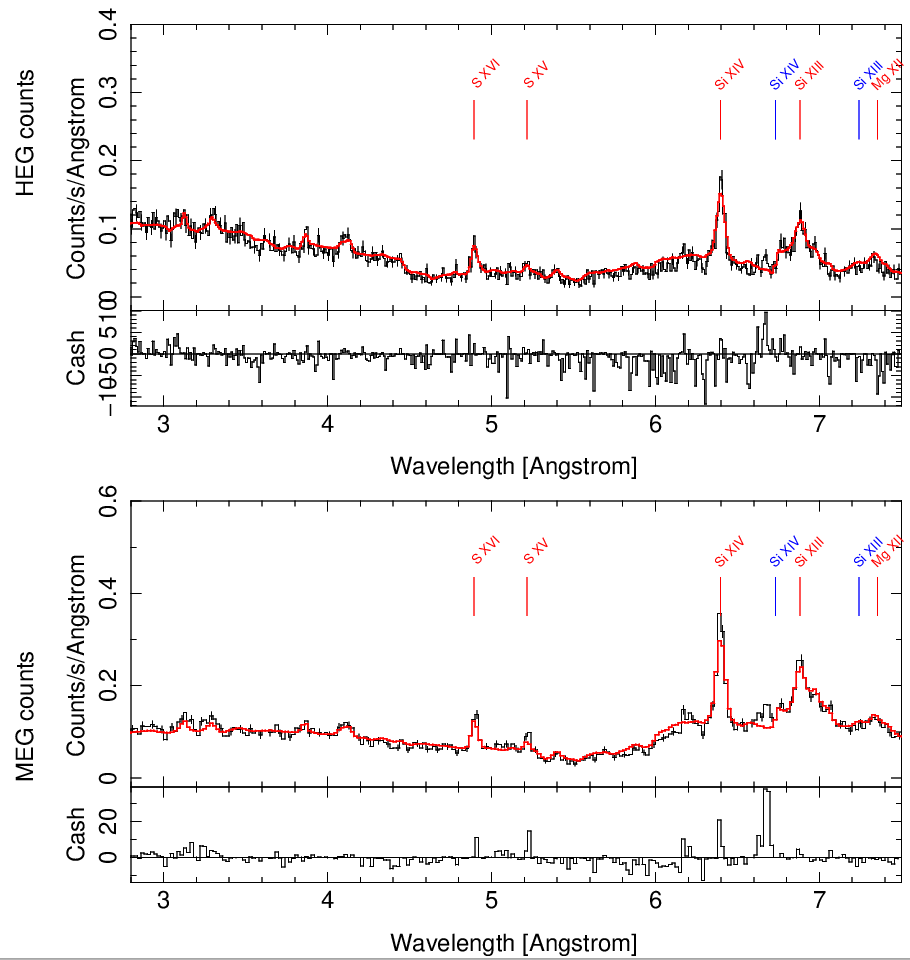
\includegraphics[width = \linewidth]{Chapters/Figures/long_plasma_whole2.png}
    \caption{Same as Figure~\ref{long_plasma1}, except for the 2.8 - 7.5 \AA\ region. }
    \label{long_plasma2}
\end{figure}


\begin{figure}
    \centering
    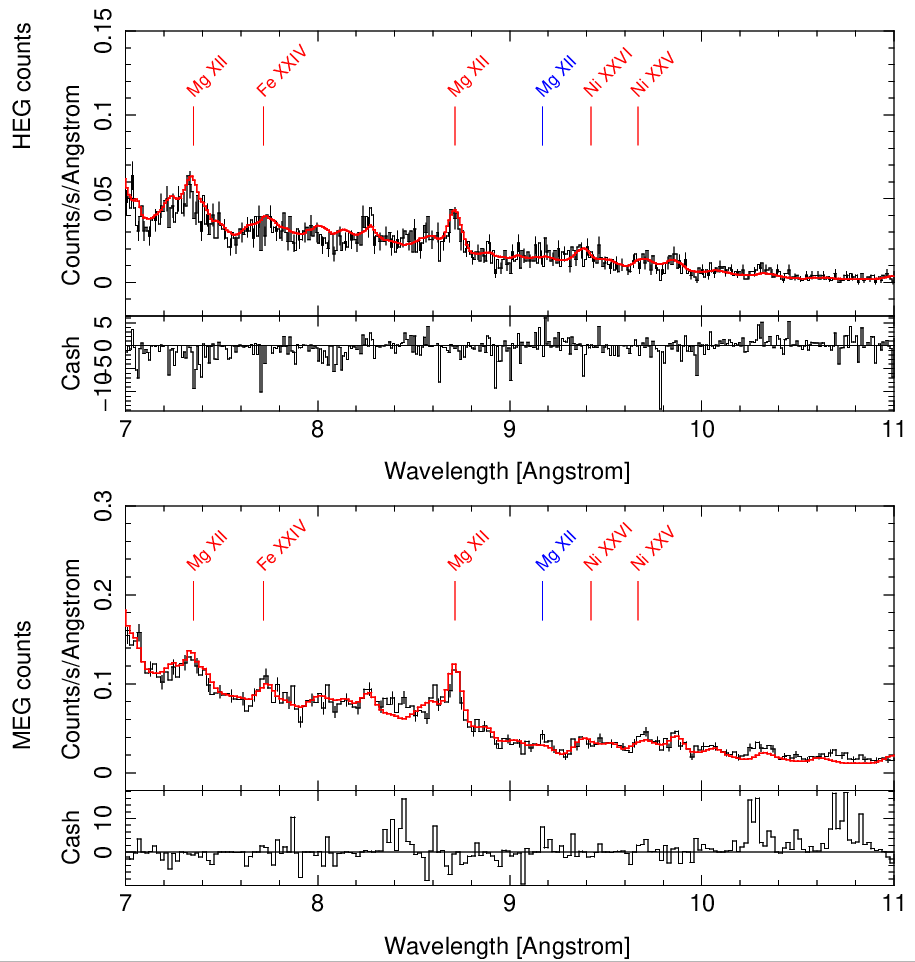
\includegraphics[width = \linewidth]{Chapters/Figures/long_plasma_whole3.png}
    \caption{Same as Figure~\ref{long_plasma1}, except for the 7-11 \AA region. }
    \label{long_plasma3}
\end{figure}













\begin{deluxetable}{rcccccc}
\tablecolumns{5}
\tablewidth{0pc}
\tabletypesize{\small}
\tablecaption{Jet Parameters from a Multitemperature model for the 100 ksec observation
\label{tab:plasma_long} }
\tablehead{& & & & &Western jet & Eastern jet\\
\colhead{T} &  \colhead{$n_e$} &  \colhead{vturb} & \colhead{metal} & \colhead{Ni} & \colhead{EM} & \colhead{EM} \\
  \colhead{($\times 10^6$ K)}  & \colhead{($\times 10^{14} \mathrnm{cm^{-3}}$)}& \colhead{(km/s)} &\colhead{($\odot$ metal)} & \colhead{($\odot$ Ni)} & \colhead{($\times 10^{57}\mathrm{cm^{-3}}$)} & \colhead{($\times 10^{57}\mathrm{cm^{-3}}$)}}
\startdata
6.3& 1 & 1662.2 & 2.79 & 30.21 & 0.58 &  0.23 \\
12.6& 1 & 1662.2& 2.79 & 30.21 & 2.09 &  $<$0.037 \\ 
31.6& 1 & 1662.2& 2.79 & 30.21 & 2.96 &  $<$0.037 \\
126.& 1 & 1662.2& 2.79 & 30.21 & 15.87 &  3.67 \\
\enddata
\end{deluxetable}





